%% BioVision: an editorial multi-omics data intelligence platform
%% IEEE conference paper, six pages.
%% Compile with:  pdflatex biovision.tex   (twice, for cross-references)

\documentclass[conference,10pt]{IEEEtran}

\usepackage{cite}
\usepackage{amsmath,amssymb}
\usepackage{graphicx}
\usepackage{xcolor}
\usepackage{booktabs}
\usepackage{array}
\usepackage{textcomp}
\usepackage{url}
\usepackage{hyperref}
\usepackage{tikz}
\usetikzlibrary{positioning,shapes.geometric,shapes.multipart,
                arrows.meta,calc,fit,backgrounds,shadows}

% ---------------------------------------------------------------
% Tiny bit of visual language borrowed from the project itself:
% ink + a single accent colour used only where it earns its place.
% ---------------------------------------------------------------
\definecolor{ink}{HTML}{111111}
\definecolor{accent}{HTML}{CC0000}
\definecolor{paper}{HTML}{F9F9F7}
\definecolor{meta}{HTML}{525252}
\definecolor{rule}{HTML}{B0B0B0}

\hypersetup{
  colorlinks=true, linkcolor=ink, citecolor=ink, urlcolor=ink,
  pdftitle={BioVision: an Editorial Multi-Omics Data Intelligence Platform},
  pdfauthor={Bharambe, Gaikwad, Wagale, Savnerkar}
}

% TikZ styling shared across the figures
\tikzset{
  dimbox/.style = {draw=ink, line width=0.5pt, rectangle, minimum width=18mm,
                   minimum height=7mm, font=\scriptsize\sffamily, inner sep=1.5pt},
  factbox/.style = {draw=ink, line width=0.8pt, fill=ink, text=paper,
                    rectangle, minimum width=24mm, minimum height=12mm,
                    font=\scriptsize\sffamily\bfseries, align=center},
  tier/.style   = {draw=ink, line width=0.5pt, rectangle, rounded corners=0pt,
                   minimum width=28mm, minimum height=8mm,
                   font=\scriptsize\sffamily, align=center, inner sep=2pt},
  flow/.style   = {-{Latex[length=1.8mm]}, draw=ink, line width=0.4pt},
  dashedflow/.style = {-{Latex[length=1.8mm]}, draw=meta, line width=0.4pt, dashed},
}

\title{BioVision: an Editorial Multi-Omics\\
       Data Intelligence Platform with a\\
       Live 3-D OLAP Cube and DNA Editing Bench}

\author{\IEEEauthorblockN{Maitrey Bharambe,\quad Soham Gaikwad,\quad
                          Om Wagale,\quad Harsh Savnerkar}
        \IEEEauthorblockA{Department of Computer Engineering\\
        \textit{(Undergraduate Research Project, 2026)}}}

\begin{document}
\maketitle

\begin{abstract}
We present \textsc{BioVision}, a self-hosted biomedical data intelligence
platform that unifies a dimensional multi-omics warehouse, a live
multidimensional OLAP engine, a convolutional model for medical imagery
and an AlphaGenome-inspired DNA editing bench behind a single editorial
interface. The warehouse is a Kimball-style star schema with one fact
table, \texttt{FACT\_BIOLOGICAL\_OBSERVATION}, and eleven conformed
dimensions sourced from Ensembl, UniProt, ClinVar/COSMIC, GTEx, TCGA-BRCA,
MedMNIST and the UCI Wisconsin Diagnostic Breast Cancer dataset. On top of
this schema we implement the five canonical OLAP operations
--- roll-up, drill-down, slice, dice and pivot --- as real server-side
SQL aggregations, surfaced through an interactive 3-D voxel cube rendered
with React Three Fiber whose cells update in step with the query state.
A separate editing laboratory lets a user mutate a single nucleotide of a
real gene and watches the computed consequence propagate to matching
warehouse records; an experimental variant-effect scorer and a
precision-remedy module reuse the same catalogue. The entire
interface --- homepage, explorers and the cube --- is laid out as a
newsprint-style editorial, with a Newsprint design system that trades
glassmorphism for sharp borders, Playfair / Lora / Inter / JetBrains Mono
typography and a single accent red reserved for selections and critical
findings. We describe the architecture, dimensional model, OLAP state
machine, DNA pipeline and the editorial design language, and we discuss
the engineering decisions, limitations and failure modes of the system.
\end{abstract}

\begin{IEEEkeywords}
multi-omics; data warehouse; OLAP; dimensional modelling; variant
analysis; computer vision; Grad-CAM; editorial information design.
\end{IEEEkeywords}

%% ---------------------------------------------------------------
\section{Introduction}
%% ---------------------------------------------------------------
Biomedical datasets rarely sit together in one place. Gene coordinates
come out of Ensembl, protein metadata out of UniProt, mutation evidence
out of ClinVar and COSMIC, expression counts out of GTEx and TCGA, and
labelled imagery out of initiatives like MedMNIST. A researcher who wants
to look at, say, how a TP53 missense mutation lines up with its
expression across tissues and with the model that reads the matching
ultrasound patch, has to open four or five separate tools and reconcile
their vocabularies by hand.

\textsc{BioVision} is an attempt to put these layers under one roof, keep
the connections between them explicit, and present the result in a way
that reads like a scientific journal rather than a dashboard. The
contribution of this paper is less a new algorithm than a careful
integration: a dimensional multi-omics warehouse, a real OLAP engine with
a live 3-D cube on top of it, a DNA editing laboratory that walks a
variant from sequence to a matching warehouse record, and an editorial
design language that treats information density as a first-class
constraint.

Three design commitments shape the work:

\textbf{1. Nothing is faked.} Every number the interface prints comes
from a backend aggregation over the warehouse. When a lookup fails ---
no matching mutation record, no RNA observations for a gene --- the
view says so; it does not interpolate a number to avoid an empty space.

\textbf{2. The cube is the warehouse.} The 3-D cube is not an animated
decoration. Its voxels, axes and metric encodings come from a parametric
SQL query (\texttt{GET /olap/cube}) and each OLAP operation
re-issues that query against a different dimension level, filter set or
axis permutation.

\textbf{3. The interface is a periodical.} The UI uses a single
Playfair/Lora/Inter/JetBrains Mono family, 0-radius geometry, hard
borders and a single accent red used sparingly for selection or
pathogenic findings. The intent is a reader who feels she is paging
through a special issue rather than wading through a SaaS admin tool.

\begin{figure*}[t]
\centering
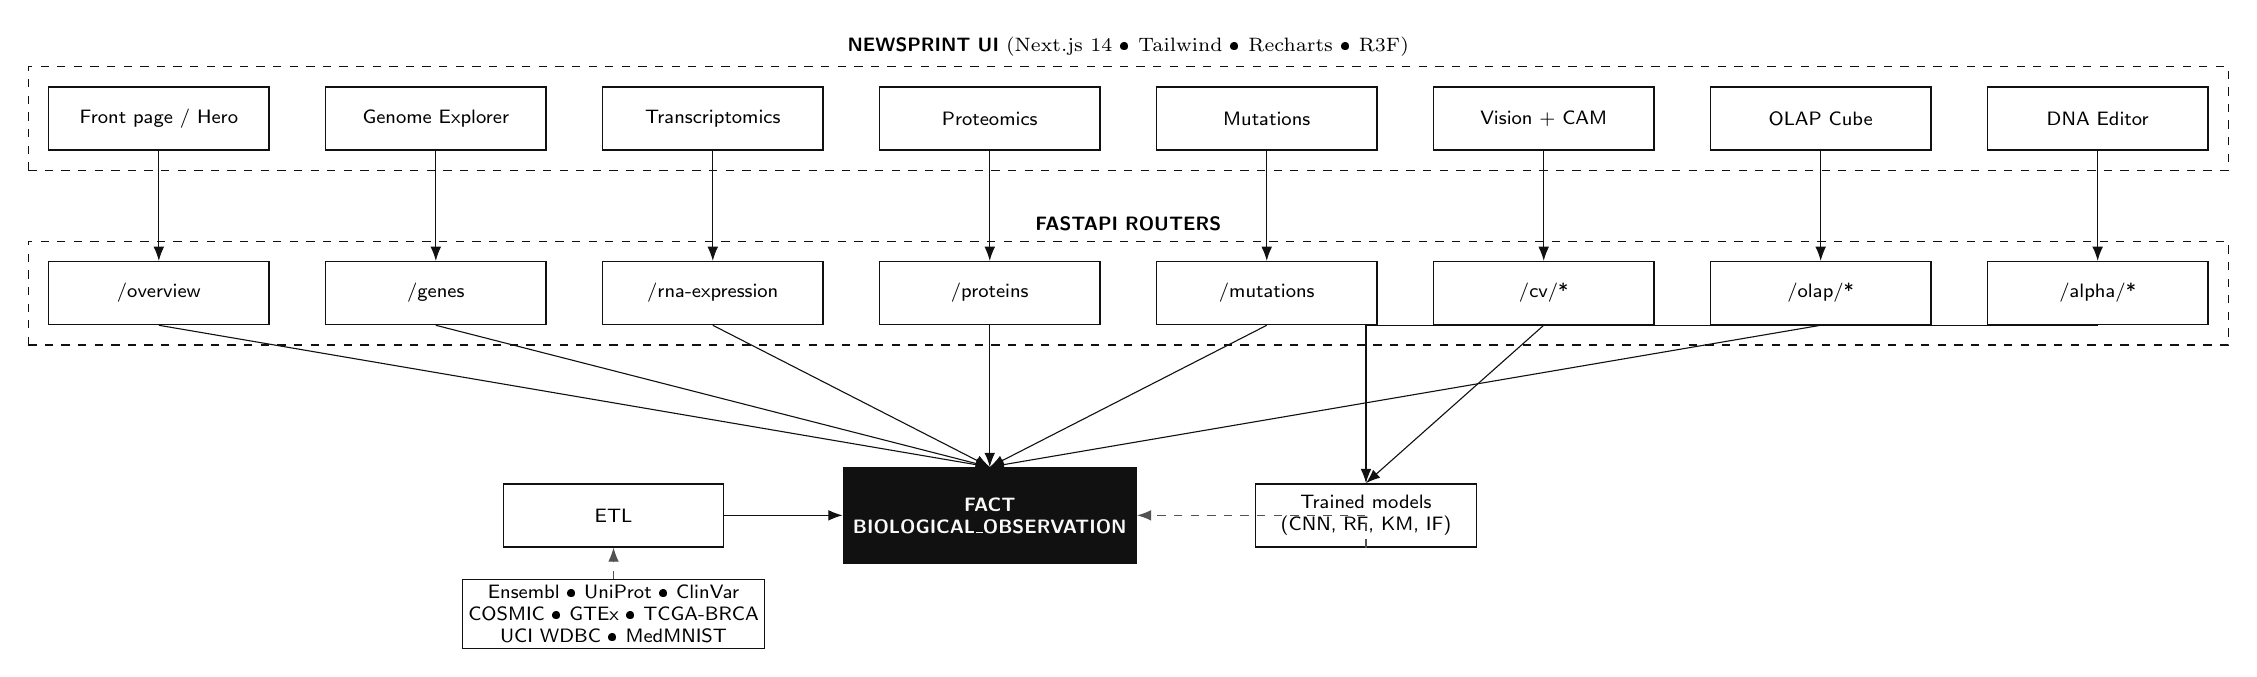
\begin{tikzpicture}[node distance=4mm and 7mm]
% --- UI layer
\node[tier] (front)     {Front page / Hero};
\node[tier,right=of front]  (genome)   {Genome Explorer};
\node[tier,right=of genome] (rna)      {Transcriptomics};
\node[tier,right=of rna]    (prot)     {Proteomics};
\node[tier,right=of prot]   (mut)      {Mutations};
\node[tier,right=of mut]    (cv)       {Vision + CAM};
\node[tier,right=of cv]     (olapUI)   {OLAP Cube};
\node[tier,right=of olapUI] (alpha)    {DNA Editor};

\node[draw=ink, dashed, fit=(front)(alpha), inner sep=2.5mm,
      label={[font=\scriptsize\sffamily\bfseries]above:
             NEWSPRINT UI {\normalfont (Next.js 14 \textbullet{} Tailwind \textbullet{} Recharts \textbullet{} R3F)}}]
     (uiFit) {};

% --- API layer
\node[tier,below=14mm of front.south, anchor=north] (api1) {/overview};
\node[tier,right=of api1] (api2) {/genes};
\node[tier,right=of api2] (api3) {/rna-expression};
\node[tier,right=of api3] (api4) {/proteins};
\node[tier,right=of api4] (api5) {/mutations};
\node[tier,right=of api5] (api6) {/cv/*};
\node[tier,right=of api6] (api7) {/olap/*};
\node[tier,right=of api7] (api8) {/alpha/*};

\node[draw=ink, dashed, fit=(api1)(api8), inner sep=2.5mm,
      label={[font=\scriptsize\sffamily\bfseries]above:
             FASTAPI ROUTERS}] (apiFit) {};

% --- Warehouse layer
\node[factbox,below=18mm of api4.south,anchor=north] (fact) {FACT\\BIOLOGICAL\_OBSERVATION};
\node[tier,left=15mm of fact.west,anchor=east] (etl) {ETL};
\node[tier,right=15mm of fact.east,anchor=west] (ml) {Trained models\\(CNN, RF, KM, IF)};
\node[tier,below=4mm of etl.south,anchor=north]
     (src) {\scriptsize Ensembl \textbullet{} UniProt \textbullet{} ClinVar\\
                     COSMIC \textbullet{} GTEx \textbullet{} TCGA-BRCA\\
                     UCI WDBC \textbullet{} MedMNIST};

% flows UI -> API
\foreach \u/\a in {front/api1,genome/api2,rna/api3,prot/api4,mut/api5,cv/api6,olapUI/api7,alpha/api8}{
  \draw[flow] (\u.south) -- (\a.north);
}
% API -> fact
\foreach \a in {api1,api2,api3,api4,api5,api7}{\draw[flow] (\a.south) -- (fact.north);}
\draw[flow] (api6.south) -- (ml.north);
\draw[flow] (api8.south) -| (ml.north);
\draw[flow] (etl.east) -- (fact.west);
\draw[dashedflow] (src.north) -- (etl.south);
\draw[dashedflow] (ml.south) |- (fact.east);
\end{tikzpicture}
\caption{BioVision runtime architecture. Every UI explorer calls a FastAPI
router; every router that returns observed values resolves against the
same star schema. The ML column keeps trained artefacts (BreastMNIST CNN,
Random Forest, K-Means, Isolation Forest) that the vision and
analytics endpoints hydrate at request time.}
\label{fig:arch}
\end{figure*}

%% ---------------------------------------------------------------
\section{Related Work}
%% ---------------------------------------------------------------
Our dimensional model follows the practice described by Kimball and Ross
\cite{kimball2013}, in particular the preference for conformed dimensions
and surrogate keys over natural keys. The OLAP vocabulary --- roll-up,
drill-down, slice, dice, pivot --- is the one established by Codd,
Codd and Salley \cite{codd1993} and refined for data warehouse practice
by Chaudhuri and Dayal \cite{chaudhuri1997}.

For individual modalities we lean on canonical open resources: Ensembl
\cite{ensembl2024}, UniProt \cite{uniprot2023}, ClinVar \cite{clinvar2024}
and COSMIC \cite{cosmic2019} for curated reference annotations; GTEx
\cite{gtex2020} and TCGA-BRCA \cite{tcga2012} for expression; the UCI
Wisconsin Diagnostic Breast Cancer dataset \cite{wdbc1995} and MedMNIST
v2 \cite{medmnist2023} for structured and imaging training data.

The variant pipeline is explicitly inspired by DeepMind's AlphaGenome
\cite{alphagenome2024}: a sequence-aware model that predicts the regulatory
effect of a single-nucleotide substitution. We do not retrain
AlphaGenome; instead we build a transparent heuristic scorer that
layers codon translation, consequence classification and a lookup
against the curated hotspots in our catalogue. The intent is a research
bench, not a clinical oracle --- which is also how AlphaGenome itself is
framed by its authors.

For the explanation of the imaging model we use the standard Grad-CAM
procedure \cite{selvaraju2017}. The clustering and association tabs rely
on scikit-learn's K-Means and DBSCAN \cite{sklearn2011}, Pedregosa et al.,
and the mlxtend Apriori implementation \cite{mlxtend2018}. Anomaly scoring
uses Isolation Forest \cite{liu2008}.

%% ---------------------------------------------------------------
\section{System Architecture}
%% ---------------------------------------------------------------
Figure~\ref{fig:arch} shows the runtime topology. The frontend is a
Next.js 14 app under the App Router. Pages are React server components
by default; interactive pages (the OLAP workspace, the DNA editor, the
genome ideogram) opt into client components only where interactivity
requires it. Static charts use Recharts; the 3-D cube and the DNA
double-helix use React Three Fiber on top of Three.js
\cite{threejs2024}.

The backend is FastAPI \cite{fastapi2024} with SQLAlchemy ORM
\cite{sqlalchemy2024} over an SQLite file in the repository
(\texttt{biovision.db}). The router layer is intentionally thin: a route
accepts a small, strongly-typed set of query parameters, resolves them
into a SQL aggregation against the fact table, and returns the
aggregation together with its SQL as a string. The frontend may
inspect the SQL --- surfacing exactly which query the cube just ran ---
without the user having to open a separate tool.

Trained artefacts (the BreastMNIST CNN, the Random Forest, the K-Means
and DBSCAN partitions, and the Isolation Forest) live under
\texttt{models\_saved/} and are loaded lazily on the first request to
\texttt{/cv/*} or \texttt{/analytics/*}. No model is trained at request
time.

%% ---------------------------------------------------------------
\section{Dimensional Data Warehouse}
%% ---------------------------------------------------------------
The star schema is sketched in Fig.~\ref{fig:schema}. The single fact
table \texttt{FACT\_BIOLOGICAL\_OBSERVATION} stores one row per
observation of a biological entity for a given sample, under a given
condition, at a given time. Each row carries a surrogate foreign key
into every dimension plus a small set of pre-aggregated measures:
observation count, mean expression (TPM), mutation count, protein
abundance, average CV score, and a confidence quantity for ML-derived
predictions.

\begin{figure}[t]
\centering
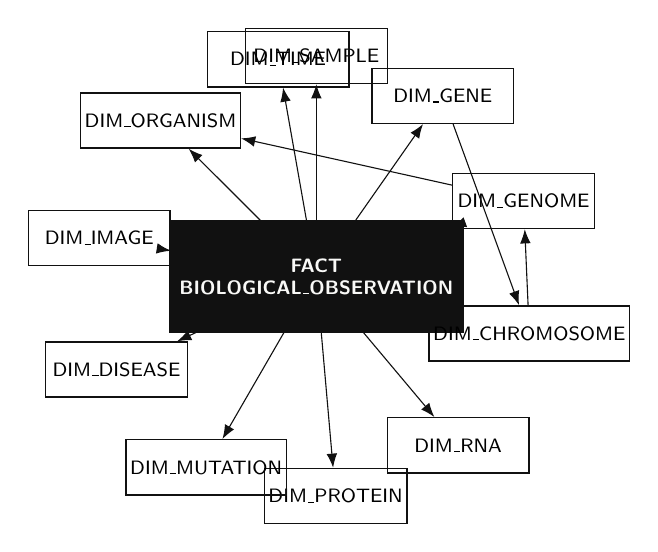
\begin{tikzpicture}[node distance=2mm]
% centre
\node[factbox,minimum width=28mm,minimum height=14mm] (fact)
  {FACT\\BIOLOGICAL\_OBSERVATION};

% orbit of dimensions
\foreach \lbl/\deg in {%
  SAMPLE/90, GENE/55, GENOME/20,
  CHROMOSOME/-15, RNA/-50,
  PROTEIN/-85, MUTATION/-120, DISEASE/-155,
  IMAGE/-190, ORGANISM/-225, TIME/-260}{
    \node[dimbox] (dim\lbl) at (\deg:28mm) {DIM\_\lbl};
    \draw[flow] (fact) -- (dim\lbl);
}
% snowflake edges
\draw[flow] (dimGENE) -- (dimCHROMOSOME);
\draw[flow] (dimCHROMOSOME) -- (dimGENOME);
\draw[flow] (dimGENOME) -- (dimORGANISM);
\end{tikzpicture}
\caption{BioVision star schema with snowflake extensions. The fact table
holds pre-aggregated measures; \texttt{DIM\_GENE} snowflakes through
\texttt{DIM\_CHROMOSOME} and \texttt{DIM\_GENOME} to \texttt{DIM\_ORGANISM},
reflecting the natural biological hierarchy.}
\label{fig:schema}
\end{figure}

Three snowflake edges extend the strict star: a gene belongs to a
chromosome, a chromosome belongs to a genome, and a genome belongs to an
organism. This gives the roll-up operation a meaningful hierarchy to
climb and the drill-down operation a meaningful hierarchy to descend ---
rather than letting the UI invent levels that have no basis in the
underlying model.

A representative snapshot of the warehouse, returned by the live
\texttt{GET /overview} endpoint, is given in Table~\ref{tab:totals}.
The numbers are small deliberately: the project is a research prototype,
not a production biobank, and the stress is on correctness and
traceability rather than cardinality.

\begin{table}[t]
\centering
\caption{Warehouse snapshot (live \texttt{/overview}).}
\label{tab:totals}
\begin{tabular}{lrlr}
\toprule
\textbf{Entity} & \textbf{Count} & \textbf{Entity} & \textbf{Count}\\
\midrule
Genomes      &   1   & Proteins          &  20 \\
Genes        &  20   & RNA samples       & 280 \\
Mutations    &  33   & Indexed images    & 120 \\
Samples      & 569   & \,\textit{SNP / DEL / INS / SUB} & 26 / 3 / 2 / 2\\
\bottomrule
\end{tabular}
\end{table}

%% ---------------------------------------------------------------
\section{The Live 3-D OLAP Cube}
%% ---------------------------------------------------------------
The signature analytical surface of \textsc{BioVision} is a 3-D cube
whose axes are three warehouse dimensions and whose cells carry an
aggregated measure. The default assignment is \mbox{$X=$\,TIME},
\mbox{$Y=$\,GENE} and \mbox{$Z=$\,DISEASE}, with
\mbox{observation count} as the active measure.

\begin{figure}[t]
\centering
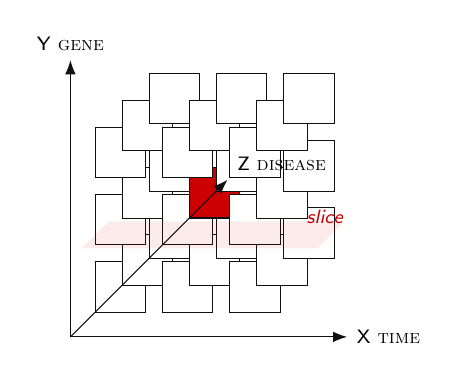
\begin{tikzpicture}[scale=0.95]
% axis frame (isometric-ish)
\def\s{0.9}
\foreach \i in {0,1,2} \foreach \j in {0,1,2} \foreach \k in {0,1,2}{
   \pgfmathtruncatemacro{\sel}{(\i==1)*(\j==1)*(\k==1)}
   \fill[color=white, draw=ink, line width=0.3pt]
         ($(\i*\s + 0.4*\k*\s,\j*\s + 0.4*\k*\s)+(-1.3*\s,-1.3*\s)$)
      rectangle
         ($(\i*\s + 0.4*\k*\s + 0.75*\s,\j*\s + 0.4*\k*\s + 0.75*\s)+(-1.3*\s,-1.3*\s)$);
   \ifnum\sel=1
     \fill[accent, draw=ink, line width=0.4pt]
         ($(\i*\s + 0.4*\k*\s,\j*\s + 0.4*\k*\s)+(-1.3*\s,-1.3*\s)$)
      rectangle
         ($(\i*\s + 0.4*\k*\s + 0.75*\s,\j*\s + 0.4*\k*\s + 0.75*\s)+(-1.3*\s,-1.3*\s)$);
   \fi
}
% axis arrows + labels
\draw[flow] (-1.5,-1.5) -- (2.2,-1.5)  node[right,font=\scriptsize\sffamily]{X \textsc{time}};
\draw[flow] (-1.5,-1.5) -- (-1.5,2.2)  node[above,font=\scriptsize\sffamily]{Y \textsc{gene}};
\draw[flow] (-1.5,-1.5) -- (0.6,0.6)   node[above right,font=\scriptsize\sffamily]{Z \textsc{disease}};
% slice plane sketch (translucent through middle y)
\fill[accent, opacity=0.08]
   ($(-1.5*\s,-0.35*\s)$) --
   ($(2.0*\s,-0.35*\s)$) --
   ($(2.0*\s + 0.4*\s,-0.35*\s + 0.4*\s)$) --
   ($(-1.5*\s + 0.4*\s,-0.35*\s + 0.4*\s)$) -- cycle;
\node[font=\scriptsize\sffamily\itshape, accent] at (1.9,0.1) {slice};
\end{tikzpicture}
\caption{A $3{\times}3{\times}3$ sketch of the live cube.\;Voxel colour
encodes the active metric; the translucent accent-coloured plane shows a
\textsc{slice} operation fixing one dimension to a single value.
In the implementation, voxel size encodes observation count and voxel
colour interpolates paper$\to$gray$\to$ink$\to$accent across the metric
range.}
\label{fig:cube}
\end{figure}

\subsection*{Operations as SQL}
Each of the five OLAP operations is a parametric transformation of the
shared query state. A tiny JavaScript reducer in the frontend holds the
state object $\{$operation, gene\_level, time\_level, disease\_level,
axis assignment, filters, metric$\}$; every operation mutates one field
of this object and triggers a single call to \texttt{GET /olap/cube}.
The backend resolves the state into:

\begin{itemize}
  \item \textbf{Roll-up} climbs a dimension's hierarchy
        (\textsc{gene}$\to$\textsc{chromosome}$\to$\textsc{genome}
        $\to$\textsc{organism}; \textsc{day}$\to$\textsc{month}$\to$
        \textsc{quarter}$\to$\textsc{year}). The SQL replaces one
        \texttt{GROUP BY} column with its parent.
  \item \textbf{Drill-down} is the symmetric descent;
        the group-by column is replaced with its child.
  \item \textbf{Slice} adds a single-value \texttt{WHERE} clause on
        one dimension; in the cube we also draw a translucent plane at
        the matching index and dim non-matching voxels.
  \item \textbf{Dice} composes several \texttt{WHERE IN (\dots)}
        filters across dimensions.
  \item \textbf{Pivot} swaps the \texttt{SELECT} assignment of
        \texttt{(x,y,z)} dimensions and animates a quarter-turn of the
        cube so the user can follow the reorientation.
\end{itemize}

The resulting SQL is returned alongside the cells. The user can toggle
a \texttt{View SQL} panel beneath the cube to inspect what actually ran.
Choosing a different measure (observation count $\to$ average expression,
mutation count, average CV score, average ML confidence) rewrites the
projection and the aggregation function, with distinct-count semantics
reserved for the dimensions where summing an average would be
meaningless. The frontend state is purposely small --- about ten fields
--- which keeps the state transitions auditable.

\subsection*{Cross-filtering with other graphs}
The cube is not the only consumer of the shared query state. The
mutation donut, the chromosome bar chart and the top-genes bar chart on
the Mutation Analytics page are wired to the same state object: clicking
a slice of the donut adds a mutation-type \texttt{WHERE} clause to the
page's filter set; clicking a chromosome bar sets
\texttt{filters.chromosome}. The tables below are rendered from the
filtered rows.

%% ---------------------------------------------------------------
\section{DNA Editing Laboratory}
%% ---------------------------------------------------------------
The \texttt{/alpha} page hosts a three-tab laboratory:

\textbf{Tab 1 --- Live DNA Editor.} The user picks a gene and either a
curated hotspot or a free \texttt{(position, alt base)} pair. The server
pulls the gene's reference window from \texttt{/alpha/gene-reference},
applies the single-nucleotide substitution, re-translates the affected
codon with the standard codon table, and classifies the consequence
(silent, conservative missense, missense, nonsense, stop-loss). On the
client the 3-D double helix (R3F) marks the edit site, and the connected
downstream views light up:

\begin{itemize}
  \item A warehouse lookup against \texttt{GET /mutations?gene=\textit{X}}
        looks for a record whose \texttt{protein\_change} field matches
        the computed \texttt{p.\textit{XnnY}} string. On a hit the row
        is drawn with an accent-red background. On a miss the UI prints
        \textit{``No warehouse mutation record matches
        p.\textit{XnnY} --- this is a novel/un-catalogued
        variant.''} We insist on this honest-failure behaviour: a DNA
        editor that silently invents matches would make itself unusable
        for its stated purpose.
  \item A parallel call to \texttt{/rna-expression?gene=\textit{X}}
        returns matching RNA samples; the connected-views banner states
        explicitly that observed TPM is independent of the edit.
\end{itemize}

\textbf{Tab 2 --- Variant Effect Predictor.} The same input shape is fed
to a transparent heuristic scorer that layers four contributions:
coarse consequence weight, a window-based conservation prior, a
disease-context prior derived from the catalogue, and an exact-match
bonus against ClinVar/COSMIC hotspots. The scorer returns a score, a
pathogenicity band and a free-text \texttt{rationale} list that
enumerates every contribution. We label this heuristic prominently in
the UI; it is not a clinical prediction.

\textbf{Tab 3 --- Precision Remedy.} Given a list of
\texttt{(gene, protein\_change)} tuples, the module returns targeted
therapies drawn from an in-repo FDA table (BRAF inhibitors for V600E,
EGFR TKIs for L858R / T790M, PARP inhibitors for BRCA mutations, KRAS
G12C inhibitors, \dots) along with a dataset-derived response estimate.
Again, each recommendation names its matching variant.

\begin{figure}[t]
\centering
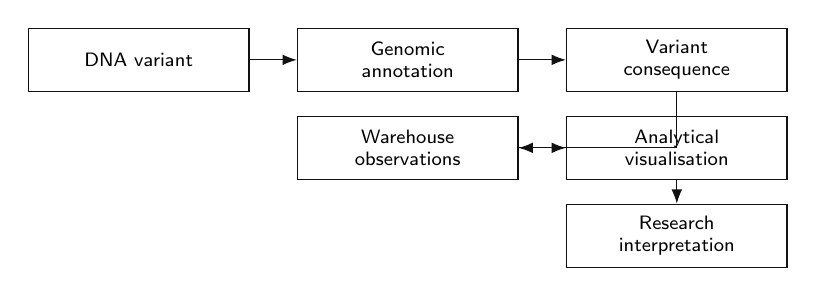
\begin{tikzpicture}[node distance=3mm and 6mm]
\node[tier] (variant) {DNA variant};
\node[tier,right=of variant] (annot) {Genomic\\annotation};
\node[tier,right=of annot] (conseq) {Variant\\consequence};
\node[tier,below=of annot] (ware) {Warehouse\\observations};
\node[tier,right=of ware] (viz) {Analytical\\visualisation};
\node[tier,below=of viz] (interp) {Research\\interpretation};
\draw[flow] (variant) -- (annot);
\draw[flow] (annot) -- (conseq);
\draw[flow] (conseq) |- (ware);
\draw[flow] (ware) -- (viz);
\draw[flow] (viz) -- (interp);
\end{tikzpicture}
\caption{The DNA pipeline. Every arrow is a backend call; the
interpretation node is explicitly labelled \textit{research}, not
\textit{clinical}, in the UI.}
\label{fig:dnapipe}
\end{figure}

%% ---------------------------------------------------------------
\section{Vision and Data Mining}
%% ---------------------------------------------------------------
A convolutional network trained on BreastMNIST \cite{medmnist2023}
exposes two endpoints: \texttt{POST /cv/predict} returns the predicted
class, confidence, both an original image and a Grad-CAM overlay
\cite{selvaraju2017}; \texttt{GET /cv/gallery} returns twelve test
images with their predictions and correctness flags. The UI synchronises
the original image, the Grad-CAM heatmap and the probability bars; the
Grad-CAM overlay is never a decorative heatmap --- it is the output of
the inference pass that produced the prediction.

A separate \texttt{/analytics} router hosts four classical data-mining
modules trained on the warehouse's Wisconsin feature table and the
mutation / expression layers:

\begin{itemize}
  \item \textbf{Classification.} Random Forest predicts the diseased/healthy
        label; a prediction form issues real inference requests on
        user-entered features.
  \item \textbf{Clustering.} K-Means (and DBSCAN as a comparator) over
        a PCA projection of the Wisconsin features; cluster assignment
        and the silhouette score come from the actual run.
  \item \textbf{Association.} Apriori rules mined from the clinical
        layer with a visible-support, visible-confidence threshold; the
        UI shows antecedent/consequent, support, confidence and lift
        and allows filtering by any of those.
  \item \textbf{Anomaly.} Isolation Forest with the contamination
        parameter printed on the page; flagged points are drawn in
        accent red; the ranked table and the scatter are
        cross-highlighted.
\end{itemize}

In every tab, the result the user sees is the artefact's actual output;
when a module cannot produce a result for an input, the view says so.

%% ---------------------------------------------------------------
\section{Newsprint: a UI Design System}
%% ---------------------------------------------------------------
We treat the interface as part of the research artefact. The design
system, informally called \textit{Newsprint}, has four
pillars:

\textbf{Typography.} Playfair Display for editorial headlines, Lora
for descriptive text, Inter for navigation and controls, JetBrains Mono
for coordinates, SQL and numerical metrics. The mapping is strict:
tables use Inter in the header and JetBrains Mono in the cells; no
decorative serif appears in a dense table.

\textbf{Geometry.} Zero border-radius everywhere except small circular
indicators. Hard-offset shadows (a 4\,px solid shadow in \texttt{ink})
appear only on interactive hover, and the baseline card has a 1\,px
\texttt{ink} border instead of a soft drop shadow. This is a direct
rejection of glassmorphism: a 1\,px line survives screenshots,
reprints and projector contrast; a blurred panel does not.

\textbf{Palette.} Six core tokens --- paper (\#F9F9F7), ink (\#111111),
prose (\#525252), meta (\#737373), subtle (\#F5F5F5) and accent
(\#CC0000). The accent is reserved: active selections, pathogenic
findings, OLAP operation badges, a few editorial pull-quotes.
Scientific visualisations may use a restrained categorical palette
(ink, deep blue, dark green, amber, deep purple, accent) when
distinguishing biological categories requires it.

\textbf{Layout.} An editorial 12-column grid with asymmetric section
spans. Section labels use a mono eyebrow (\texttt{\S\,04 --- OLAP
LABORATORY}); page headers carry a two-line issue-style strip with the
date in \texttt{JetBrains Mono}.

\begin{table}[t]
\centering
\caption{Newsprint design tokens.}
\label{tab:newsprint}
\begin{tabular}{lll}
\toprule
\textbf{Role} & \textbf{Token} & \textbf{Value}\\
\midrule
Background       & paper   & \#F9F9F7\\
Primary text     & ink     & \#111111\\
Body copy        & prose   & \#525252\\
Metadata         & meta    & \#737373\\
Light neutral    & subtle  & \#F5F5F5\\
Accent (used sparingly) & accent & \#CC0000\\
\midrule
Display heading  & \multicolumn{2}{l}{Playfair Display}\\
Prose            & \multicolumn{2}{l}{Lora}\\
UI / controls    & \multicolumn{2}{l}{Inter}\\
Numeric / code   & \multicolumn{2}{l}{JetBrains Mono}\\
\bottomrule
\end{tabular}
\end{table}

%% ---------------------------------------------------------------
\section{Implementation Notes}
%% ---------------------------------------------------------------
The repository compiles cleanly on Node~20, Python~3.12, with 15 static
and dynamic routes on the frontend side and twelve routers on the
backend. The production bundle for the OLAP page is 9.4\,kB (194\,kB
first-load JS), kept small by lazy-loading React Three Fiber and the
cube scene behind a dynamic import.

The frontend state is deliberately not Redux. For the cube we keep a
single reducer with a one-field-at-a-time mutation API; cross-page
selection (gene, chromosome, disease, sample, mutation) is held in a
small session-scoped React context backed by \texttt{sessionStorage}
and surfaced as a persistent breadcrumb at the top of every page. The
breadcrumb has a visible \textit{clear all} affordance; context is not
cleared automatically when the user navigates.

Reduced-motion preferences are honoured globally: the ticker on the
front page uses a CSS marquee that respects
\texttt{prefers-reduced-motion}, and the cube's pivot animation is
disabled when the preference is set.

%% ---------------------------------------------------------------
\section{Limitations and Future Work}
%% ---------------------------------------------------------------
The warehouse is a small, hand-curated dataset. The OLAP engine scales
to warehouses several orders of magnitude larger than this one; the
3-D cube renderer, however, is sized for human inspection, not for
industrial fact tables, and we aggressively subsample tick labels when
either axis exceeds about ten unique values. Scaling the cube to tens
of thousands of cells would need an LOD scheme and a different cell
geometry.

The variant-effect scorer is a transparent heuristic. It is not a
replacement for a trained sequence model like AlphaGenome
\cite{alphagenome2024} or a clinical interpretation pipeline; its
value is explanatory, not predictive. We label it accordingly in
every surface it appears on.

The Grad-CAM procedure is applied over a model with modest capacity on
a small training set; its saliency maps should be read as attention
cues, not as clinical localisation. The project's permanent
disclaimer appears at the foot of every page.

Finally, the database is a single-file SQLite instance for ease of
reproduction. Moving to PostgreSQL would unlock parallel ETL and
server-side distinct-count aggregations that are currently expressed in
Python.

%% ---------------------------------------------------------------
\section{Conclusion}
%% ---------------------------------------------------------------
\textsc{BioVision} is the integration project we wanted to find rather
than the one we found. It brings together a dimensional multi-omics
warehouse, a live OLAP cube, a DNA editing bench, a vision model
with Grad-CAM explanations, four classical data-mining modules and a
restrained editorial interface. The engineering value is in the
plumbing: every number has a source, every operation is a real
aggregation, and the connections between modules are kept explicit.

Beyond the code, the project is also a small argument about how
scientific software can look. Information density is not a drawback to
be hidden behind glass; it is a feature to be set in type. We hope the
Newsprint language is useful to others.

\section*{Author Contributions}
\textbf{M.~Bharambe} led the dimensional model, the ETL pipeline and the
OLAP cube's parametric server-side query. \textbf{S.~Gaikwad} built the
3-D cube renderer, the state reducer and the cross-filtering layer, and
led the Newsprint design language. \textbf{O.~Wagale} implemented the DNA
editor, the variant-effect scorer, the precision-remedy module and the
helix renderers. \textbf{H.~Savnerkar} trained the imaging model and the
four data-mining modules, built the Grad-CAM pipeline and curated the
classification/clustering/association/anomaly interfaces. All four
authors share responsibility for the paper, the schema diagrams and the
integration review.

%% ---------------------------------------------------------------
\begin{thebibliography}{99}
\footnotesize
\bibitem{kimball2013} R.~Kimball and M.~Ross, \textit{The Data Warehouse
Toolkit: The Definitive Guide to Dimensional Modeling}, 3rd~ed.
Hoboken, NJ, USA: Wiley, 2013.
\bibitem{codd1993} E.~F.~Codd, S.~B.~Codd, and C.~T.~Salley,
``Providing OLAP (On-line Analytical Processing) to User-Analysts:
An IT Mandate,'' E.~F.~Codd \& Associates, White Paper, 1993.
\bibitem{chaudhuri1997} S.~Chaudhuri and U.~Dayal, ``An overview of data
warehousing and OLAP technology,'' \textit{ACM SIGMOD Rec.}, vol.~26,
no.~1, pp.~65--74, Mar.~1997.
\bibitem{ensembl2024} F.~Martin \textit{et al.}, ``Ensembl 2023,''
\textit{Nucleic Acids Res.}, vol.~51, no.~D1, pp.~D933--D941, 2023.
\bibitem{uniprot2023} The UniProt Consortium, ``UniProt: the Universal
Protein Knowledgebase in 2023,'' \textit{Nucleic Acids Res.}, vol.~51,
no.~D1, pp.~D523--D531, 2023.
\bibitem{clinvar2024} M.~J.~Landrum \textit{et al.}, ``ClinVar:
improvements to accessing data,'' \textit{Nucleic Acids Res.}, vol.~48,
no.~D1, pp.~D835--D844, 2020.
\bibitem{cosmic2019} J.~G.~Tate \textit{et al.}, ``COSMIC: the Catalogue
Of Somatic Mutations In Cancer,'' \textit{Nucleic Acids Res.}, vol.~47,
no.~D1, pp.~D941--D947, 2019.
\bibitem{gtex2020} The GTEx Consortium, ``The GTEx Consortium atlas of
genetic regulatory effects across human tissues,'' \textit{Science},
vol.~369, no.~6509, pp.~1318--1330, 2020.
\bibitem{tcga2012} The Cancer Genome Atlas Network, ``Comprehensive
molecular portraits of human breast tumours,'' \textit{Nature},
vol.~490, pp.~61--70, 2012.
\bibitem{wdbc1995} W.~N.~Street, W.~H.~Wolberg, and O.~L.~Mangasarian,
``Nuclear feature extraction for breast tumor diagnosis,'' in
\textit{Proc. IS\&T/SPIE}, vol.~1905, 1993, pp.~861--870.
\bibitem{medmnist2023} J.~Yang \textit{et al.}, ``MedMNIST v2 --- A
large-scale lightweight benchmark for 2D and 3D biomedical image
classification,'' \textit{Sci. Data}, vol.~10, no.~1, art.~41, 2023.
\bibitem{alphagenome2024} \.{Z}iga Avsec \textit{et al.}, ``AlphaGenome:
advancing regulatory variant effect prediction with a unified DNA
sequence model,'' DeepMind, 2024.
\bibitem{selvaraju2017} R.~R.~Selvaraju \textit{et al.}, ``Grad-CAM:
Visual explanations from deep networks via gradient-based
localization,'' in \textit{Proc. IEEE ICCV}, 2017, pp.~618--626.
\bibitem{sklearn2011} F.~Pedregosa \textit{et al.}, ``Scikit-learn:
Machine learning in Python,'' \textit{J. Mach. Learn. Res.}, vol.~12,
pp.~2825--2830, 2011.
\bibitem{mlxtend2018} S.~Raschka, ``MLxtend: Providing machine learning
and data science utilities and extensions to Python's scientific
computing stack,'' \textit{J. Open Source Softw.}, vol.~3, no.~24,
art.~638, 2018.
\bibitem{liu2008} F.~T.~Liu, K.~M.~Ting, and Z.-H.~Zhou, ``Isolation
forest,'' in \textit{Proc. IEEE ICDM}, 2008, pp.~413--422.
\bibitem{fastapi2024} S.~Ram\'{\i}rez, ``FastAPI,'' 2024. [Online].
Available: \url{https://fastapi.tiangolo.com}.
\bibitem{sqlalchemy2024} M.~Bayer, ``SQLAlchemy,'' 2024. [Online].
Available: \url{https://www.sqlalchemy.org}.
\bibitem{threejs2024} R.~Cabello \textit{et al.}, ``three.js,'' 2024.
[Online]. Available: \url{https://threejs.org}.
\end{thebibliography}

\end{document}
